\section{Examples}
\label{sec:examples}
We implemented the above smooth approximation to the semantics of MTL, and tested them empirically on a number of examples.

\subsection{Approximation error for Robustness}
\label{sec: ex apx error}
\begin{figure}[t]
\centering
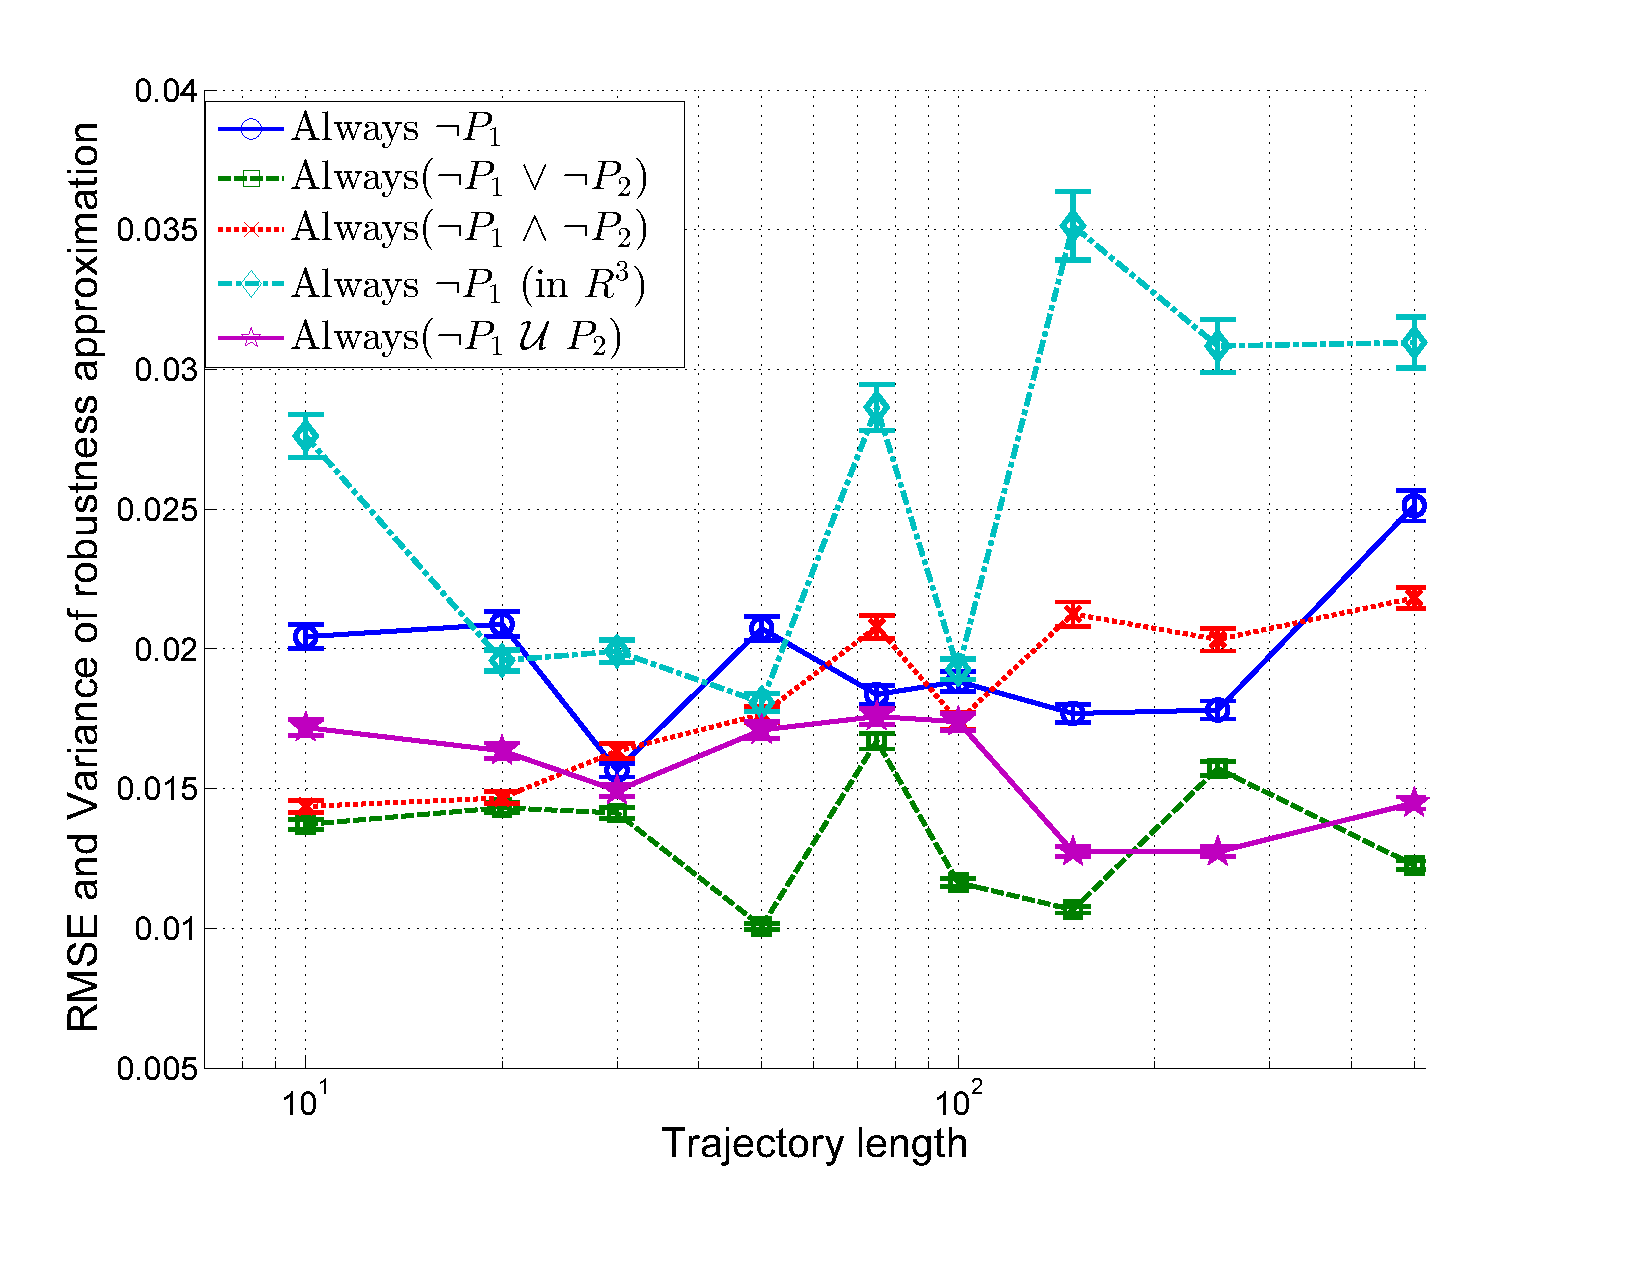
\includegraphics[width=0.49\textwidth]{figures/RobustnessError}
\caption{RMSE of approximation error for robustness with varying trajectory lengths for multiple formulae.}
\label{fig:sample result}
\end{figure}
%\todo[inline]{Yash, Show these results}

In order to study the quality of approximation empirically, we evaluated robustness and its approximation for multiple formulae for 1000 random trajectories (of varying lengths) generated for a system with 2-states and point-mass dynamics (see \eqref{eq:PointMass}) with input and state saturation. We also evaluate a single formula, for a 3-state point mass system, to observe the approximation errors in a higher dimension. Here, in all formulae, $P1$ is defined as $x \in [-1,1]^2$, and $P2$ as $x\in [2,2.5]^2$ (and similarly in $\mathbb{R}^3$). The states are constrained to be in $[-5,5]^2$ and the inputs in $[-0.3,0.3]^2$. 

Fig. \ref{fig:sample result} shows the Root Mean Square (RMSE) and variance of approximation errors $\robf-\srobf$ to give an idea of the magnitude of the approximation errors for multiple formulae. 
It is expected, and seen to some extent in Fig. \ref{fig:sample result}, that (for a constant number of wavelet coefficients) approximation error will grow as trajectory length grows. This is due to the smooth max and min functions, as seen in \eqref{eq:smooth max error}.

Fig. \ref{fig:relative error} shows the relative approximation errors, $(\robf-\srobf)/|\robf|$, for the formulae under consideration. It is seen that the relative average approximation is less than $10\%$ for all cases. 

For some data points in Fig. \ref{fig:relative error}, the variance of relative error is high, suggesting that the approximation errors vary \todo[inline]{bigly}. This is not true, as it is worth noting in Fig. \ref{fig:sample result} that the variance of the actual approximation is very small. The high relative approximation errors are due to trajectories which have a true robustness of near zero, leading to a spike in the relative approximation error, $(\robf-\srobf)/|\robf|$, even for small values of the true approximation error, $\robf-\srobf$.

Also while Fig.\ref{fig:sample result} suggests that the approximation error grows as dimension of the state grows from $2$ to $3$, Fig. \ref{fig:relative error} shows that the relative approximation error is still small. 
%As explained in the previous section, better approximation can be achieved by increasing the number of wavelet coefficients as dimension, and trajectory length, grow.
%\todo[inline]{Is that true?}

\begin{figure}[t]
\centering
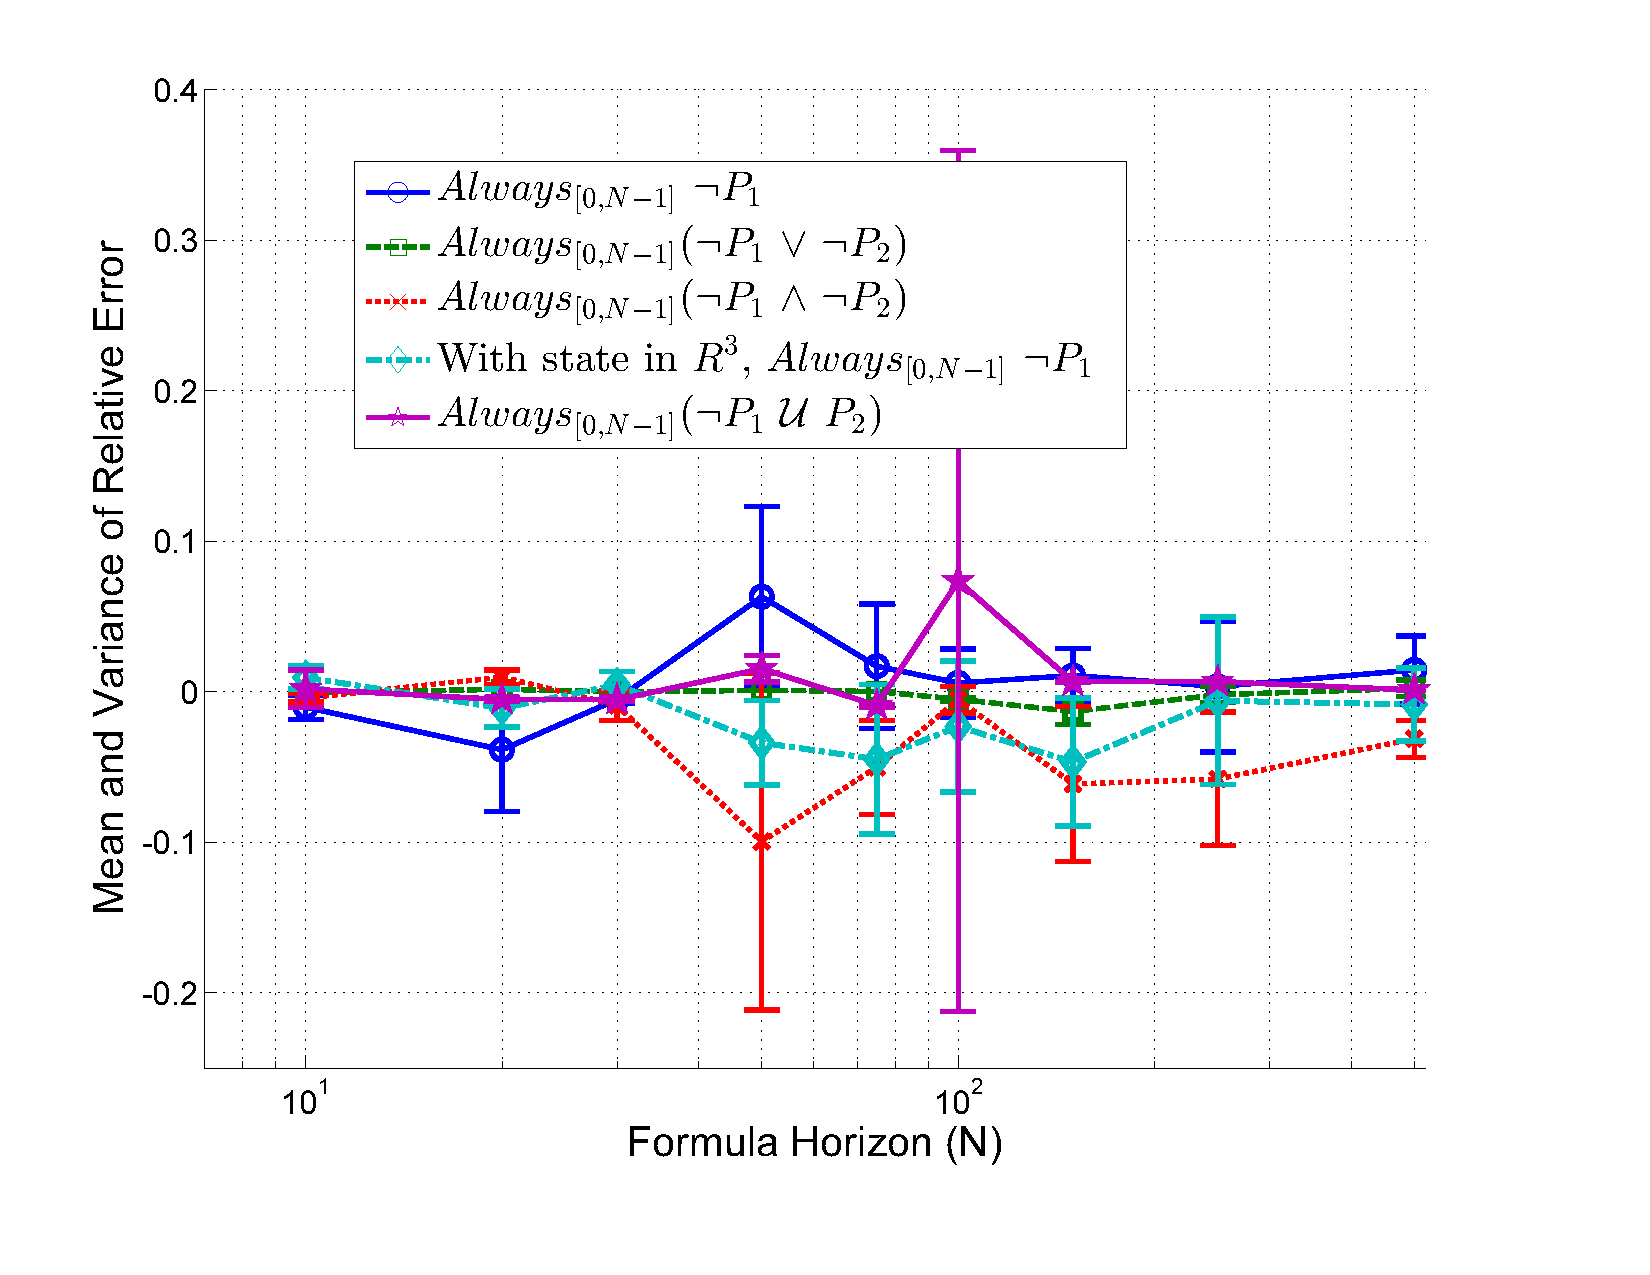
\includegraphics[width=0.49\textwidth]{figures/RobustnessErrorRel}
\caption{Mean and Variance of relative approximation error for robustness with varying trajectory lengths for multiple formulae.}
\label{fig:relative error}
\end{figure}


\subsection{Robustness maximization for control}
\label{sec:toy example}
\todo[inline]{Yash, Show SA and SR-SQP on toy example}
%Toy example text
%\todo[inline]{I expect to see first the general control problem 13a-13e, then the specific example. This way, if you define once here, we dnot have to worry about re-defining the control problem later. So: here;s the general control problem; here's a simple system.}

The control problem we solve is a generalized version of \eqref{eq:min rob problem} (using the smooth version of robustness), given by
\begin{subequations}
\label{eq:general_ctrl}
\begin{align}
\text{max } & \srob_{\formula}(\sstraj) - \gamma \sum_{k=0}^{N-1} l(x_{k+1},u_{k}) \\
\text{s.t. } & x_{k+1} = f(x_k,u_k), \, \forall k=0,\dotsc,N-1 \\
 & x_k \in X, \, \forall k=0,\dotsc,N \\
 & u_k \in U, \, \forall k=0,\dotsc,N-1 \\
 & \delta \srob_{\formula}(\sstraj) \geq 0
\end{align}
\end{subequations}
%\todo[inline]{stick to $\formula$ for a formula, not $\formula$ (unless there's a good reason)}

If we set $\gamma=0$ and $\delta=0$, we recover the problem in \eqref{eq:min rob problem} with the smooth robustness in the cost function. In the above formulation, $l(x_{k+1},u_{k})$ is a system specific control cost, e.g. the LQR cost $x_k'Qx_k + u_k'Ru_k$. $X$ and $U$ define constraints on the state $x$ and control $u$ respectively. 

For illustrative purposes, we choose a simple linear system (point-mass dynamics) to first illustrate our method. The point-mass system has the following dynamics:
\begin{equation}
\label{eq:PointMass}
x_{k+1} = x_k + u_k
\end{equation}

For the point-mass example, we define the specification to be followed as $\formula = \always_{[0,20]} \neg (x_k \in \text{Unsafe}) \land \eventually_{[0,20]} (x_k \in \text{Terminal})$, with the sets $\text{Unsafe}=[-1,1]^2$ and $\text{Terminal}=[2,2.5]^2$. In addition, for the control problem, $X=[-2.5,2.5]^2$, $U=[0.3,0.3]^2$, $\delta=1$, and we optimize for two different values of $\gamma$, $0.1$ and $0.001$, and start with an initial point $x_0=[-2,-2]'$. The control cost is $l(x_k) = ||x_k||_{2}^2$, which when summed over is the square of the trajectory length. Note, $N=21$, which is the horizon length of the specification.

An initial trajectory starting from $x_0$ and ending in the $\text{Terminal}$ set is obtained via solving a linear program for feasibility with the system dynamics and input/state constraints, and the terminal set added as a constraint. This trajectory is used as an initial point to initialize the optimization.

We use MATLAB's Sequential Quadratic Programming (SQP) solver for the optimization, and also compute a gradient for $\srob$ to be used in SQP.
%\todo[inline]{confusing...you throw around things casually like $\min 0$, as if you're daring the reader to get confused. Or "This trajectory is used to initialize the SQP optimization, which is used for the optimization."..Take your time. explain it once, well, and then forget about it. this is the \textit{illustrative} example. see my comment in ATC case study.}
\todo[inline]{say a word or two about SQP: broadly, how it works and whether it has guarantees. after all, it is to use things like SQP that we are smoothing in the first place. }

Fig.~\ref{fig:toy control} shows the sets, initial trajectory (which is unsafe and has a robustness of $-1$), and the two trajectories for the two values of $\gamma$. Both trajectories satisfy the specification $\formula$. Intuitively, the trajectories in Fig.\ref{fig:toy control} make sense, as for a higher value of $\gamma=0.1$ we get a shorter trajectory, which is closer to unsafe set, hence satisfies $\formula$ less robustly ($\rob_{\formula}=0.6543$) and for a smaller value of $\gamma=0.001$ we get a longer trajectory which has a higher robustness ($\rob_{\formula}=1.2073$).

\begin{figure}[t]
\centering
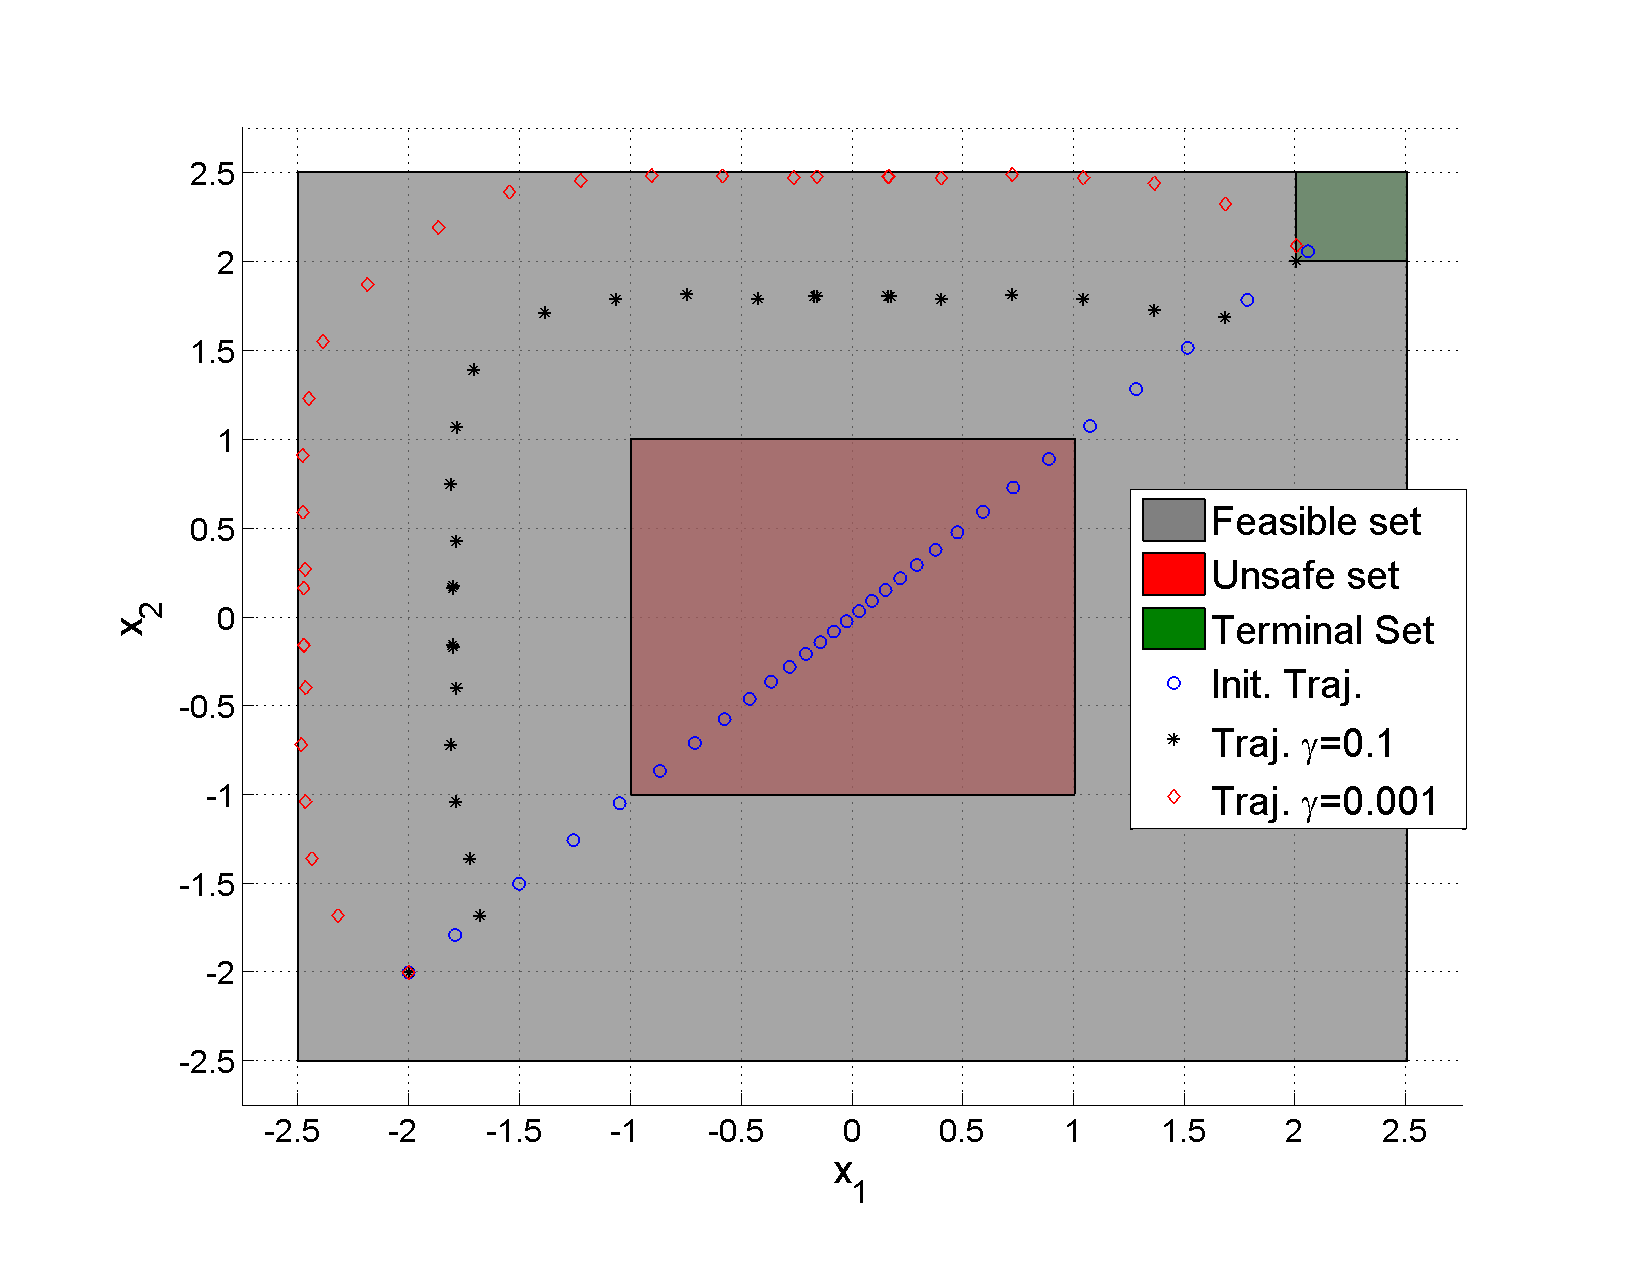
\includegraphics[width=0.49\textwidth]{figures/ToyExampleControl}
\caption{Initial trajectory and trajectories obtained for two different values of $\gamma$ in \eqref{eq:general_ctrl}.}
\label{fig:toy control}
\end{figure}

\subsection{Robustness minimization for falsification}
\label{sec:toy falsification}
\todo[inline]{Yash, Show the falsification figure for an autonomous system, comparing Method, DumbSqp,SA}
%Toy Falsification example



\begin{figure}[t]
\centering
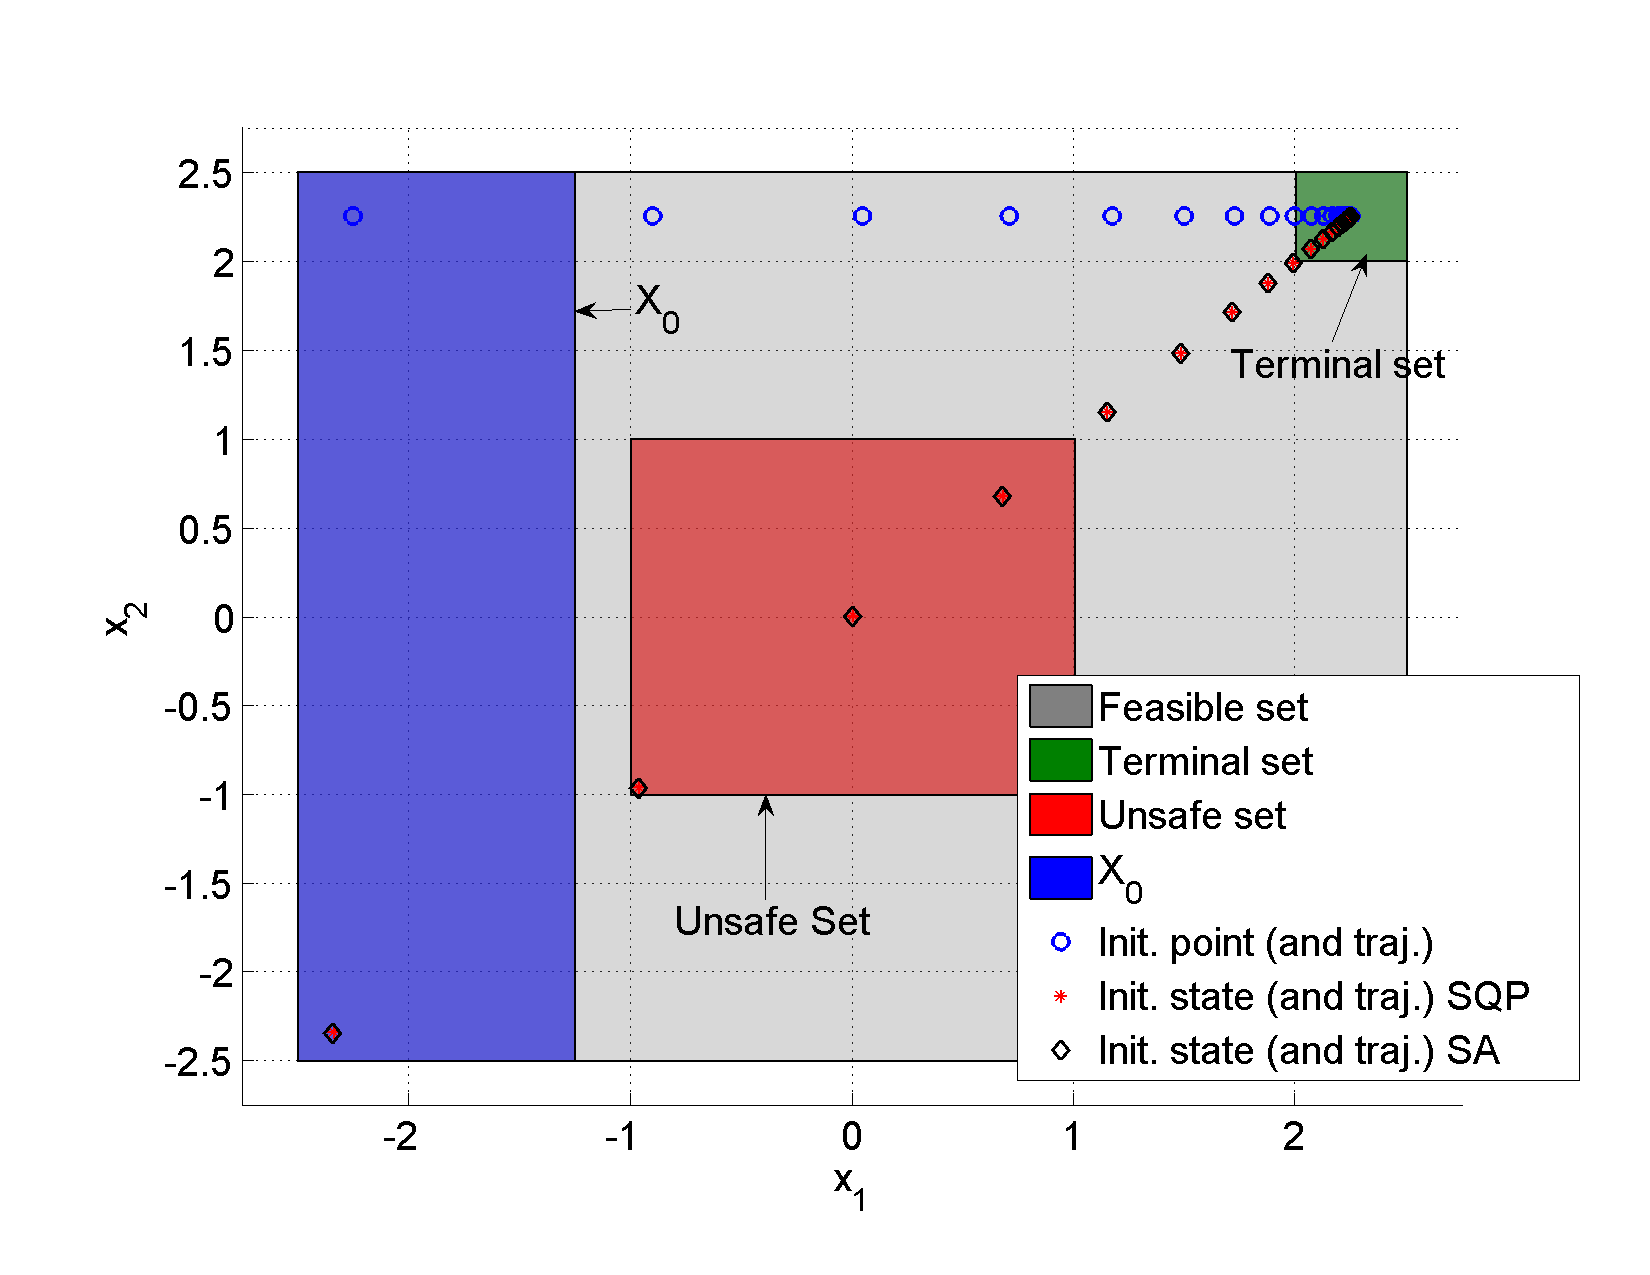
\includegraphics[width=0.49\textwidth]{figures/ToyExampleFalse}
\caption{Trajectories from initial points obtained from robustness minimization via Simulated Annealing (SA), SQP, and SQP on smooth robustness. Note, both SQP and SQP on smooth robustness lead to the same solution.}
\label{fig:toy falisification}
\end{figure}